\documentclass[12pt]{article}
\def\activityid{F10-U-v2}\usepackage[letterpaper,margin=.65in,top=.60in,bottom=.65in]{geometry}
\usepackage[T1]{fontenc}
\usepackage[default]{sourcesanspro}
\usepackage{microtype,tikz,array,tabularx,fancyhdr,amsmath,amssymb}
\usepackage[hidelinks]{hyperref}
\usetikzlibrary{calc,arrows.meta}
\setlength{\parindent}{0pt}\setlength{\parskip}{7pt}
\setlength{\headheight}{0pt}\setlength{\footskip}{26pt}\setlength{\emergencystretch}{2em}
\pagestyle{fancy}\fancyhf{}\renewcommand{\headrulewidth}{0pt}\renewcommand{\footrulewidth}{.4pt}
\fancyfoot[L]{\scriptsize Bellingham Math Circle / Week 10 / \activityid}
\fancyfoot[R]{\scriptsize \thepage}
\definecolor{ink}{gray}{.12}\definecolor{soft}{gray}{.95}\color{ink}
\newcommand{\PageTitle}[2]{{\fontsize{10}{12}\selectfont\bfseries WEEK 10\quad ROUTE LAB\hfill #1\par}\vspace{3pt}{\fontsize{26}{29}\selectfont\bfseries #2\par}\vspace{2pt}}
\newcommand{\NameLine}{{\small Name: \rule{2.65in}{.4pt}\hfill Date: \rule{1.35in}{.4pt}\par}\vspace{4pt}}
\newcommand{\Task}[2]{\par\vspace{3pt}{\large\bfseries #1}\par #2\par}
\newcommand{\Subhead}[1]{\par\vspace{3pt}{\large\bfseries #1}\par}
\newcommand{\RuleBox}[1]{\par\begingroup\setlength{\fboxsep}{8pt}\colorbox{soft}{\parbox{\dimexpr\linewidth-16pt\relax}{#1}}\endgroup\par}
\newcommand{\WriteBox}[2]{\par\textbf{#1}\par\vspace{2pt}\begin{tikzpicture}\draw[black!40,line width=.5pt] (0,0) rectangle (\dimexpr\linewidth-.5pt\relax,#2);\end{tikzpicture}\par}
\newcommand{\StudentFooter}{\vfill{\small Try it with objects. Explain by pointing, talking, or drawing.}\par}
\newcommand{\RookBoard}[3]{\begin{tikzpicture}[x=#3,y=#3]\draw[step=1,black!45] (0,0) grid (#1,#2);\draw[thick] (0,0) rectangle (#1,#2);\node[font=\Large] at ({#1-.5},.5){$\star$};\draw[-{Latex},thick] (0,-.35)--(#1,-.35);\draw[-{Latex},thick] ({#1+.35},#2)--({#1+.35},0);\end{tikzpicture}}
\newcommand{\Table}[3]{\begin{tikzpicture}[x=#3,y=#3]\draw[step=1,black!25] (0,0) grid (#1,#2);\draw[thick] (0,0) rectangle (#1,#2);\fill (0,0)circle(3pt);\draw[-{Latex},very thick] (0,0)--(.7,.7);\node[below] at ({#1/2},-.1){width #1};\node[rotate=90,above] at (-.2,{#2/2}){height #2};\end{tikzpicture}}
\newcommand{\GraphNodes}{\coordinate(A)at(0,0);\coordinate(B)at(3,0);\coordinate(C)at(1.5,2.6);\coordinate(D)at(1.5,.95);}
\newcommand{\Kfour}[1]{\begin{tikzpicture}[scale=#1]\GraphNodes\draw[very thick](A)--(B)--(C)--(A)--(D)--(B) (D)--(C);\foreach \n in {A,B,C,D}{\node[circle,draw,fill=white,minimum size=22pt,font=\bfseries]at(\n){\n};}\end{tikzpicture}}
\newcommand{\House}[1]{\begin{tikzpicture}[scale=#1]\coordinate(A)at(0,0);\coordinate(B)at(3,0);\coordinate(C)at(3,2);\coordinate(D)at(0,2);\coordinate(E)at(1.5,3.3);\draw[very thick](A)--(B)--(C)--(D)--(A) (D)--(E)--(C);\foreach \n in {A,B,C,D,E}{\node[circle,draw,fill=white,minimum size=22pt,font=\bfseries]at(\n){\n};}\end{tikzpicture}}

\begin{document}

\PageTitle{GRADES 4--5}{When does a whole-map walk exist?}\NameLine
\RuleBox{An Euler trail uses every edge exactly once, without jumping. A \textbf{closed} Euler trail returns to its start. Vertices may be revisited. Our maps are connected: every edge belongs to the same reachable network.}
\Task{1. Try the house.}{Find an Euler trail on the left map. Count edges at each vertex. Why must its endpoints be C,D? Why can it not close?}
\begin{center}
\begin{minipage}{.43\linewidth}\centering\House{.78}\end{minipage}\hfill
\begin{minipage}{.52\linewidth}\centering
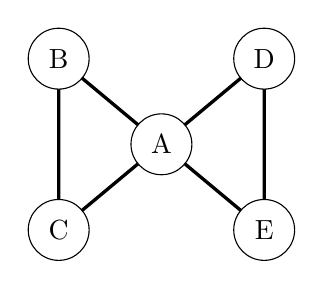
\begin{tikzpicture}[scale=.87]
\coordinate(A)at(0,0);\coordinate(B)at(-1.5,1.25);\coordinate(C)at(-1.5,-1.25);\coordinate(D)at(1.5,1.25);\coordinate(E)at(1.5,-1.25);
\draw[very thick](A)--(B)--(C)--(A)--(D)--(E)--(A);
\foreach\n in{A,B,C,D,E}{\node[circle,draw,fill=white,minimum size=22pt]at(\n){\n};}
\end{tikzpicture}
\end{minipage}
\end{center}
\Task{2. Insert a loop with your hands.}{On the right map, walk A--B--C--A, marking used roads. Another loop remains! Write A--B--C--A on one paper strip and A--D--E--A on another. At a visit to A, insert the second route into the first. Walk your joined route: did it use all six roads once?}
\WriteBox{My joined route:}{.45in}
\textbf{Optional proof conversation.} On any connected all-even map, follow unused edges until stuck. Why can that happen only at the start? If roads remain, why does some vertex on your closed walk touch one? Start another loop there and insert it. Why must this finish?

\textbf{Exactly two odd vertices?} Add one temporary edge between them. Build a closed route in the all-even map, then cut the route at that edge and remove it. What are the endpoints of the remaining route?
\StudentFooter

\newpage

\PageTitle{GRADES 4--5}{The shortest delivery round}\NameLine
\RuleBox{Now deliver along every road \textbf{at least once} and return to the start. Reusing roads is allowed. Each road costs 1 step. Minimize total steps. D is a real junction; each drawn segment is a separate road.}
\begin{center}\Kfour{1.8}\end{center}
\Task{3. Find a good route.}{Start at A. Record the vertices you visit and count steps. Can you improve your first route?}
\WriteBox{My best complete route and its length:}{.90in}
\Task{4. Prove nobody can beat it.}{There are six roads. All four vertices have odd degree. Think of each repeated crossing as adding a second copy of that road. How many odd vertices can one added copy change?}
\WriteBox{A lower bound that matches my route:}{1.0in}
\StudentFooter

\newpage

\PageTitle{GRADES 4--5}{Turn a route into an algorithm}\NameLine
\Task{5. Repair the odd vertices in pairs.}{List all ways to split A, B, C, D into two pairs. For each pairing, duplicate the road joining each pair. What happens to every degree? Why does a closed Euler trail now exist?}
\begin{center}\renewcommand{\arraystretch}{1.8}\begin{tabular}{c|p{2in}|p{2in}}Pairing&Repeated roads&Total length\\\hline1&&\\2&&\\3&&\end{tabular}\end{center}
\Task{6. Must the walk be closed?}{The mail truck may finish anywhere now. What is the fewest steps needed to visit every road? Build a route and prove its length is best.}
\WriteBox{My open route and matching lower bound:}{1.0in}
\Task{7. Become a puzzle designer.}{Draw a connected map with \textbf{six odd vertices}. Join different dots; parallel roads are allowed. Every road costs 1. Can you design one whose shortest closed delivery round needs exactly three extra steps? Save a route and a lower-bound argument with your puzzle.}
\WriteBox{A design, or the key idea I will test:}{1.0in}
\StudentFooter

\end{document}
